\section{System Overview}

\begin{outline}
  Present a high-level overview of your proposed control framework, likely including a block diagram (similar to Figure 1 in the proposal) and a description of each component.
\end{outline}

This work aims to take ContactNet \cite{bratta_contactnet_2024} and extend it to provide dynamic gait generation capabilities. ContactNet is able to generate acyclic gaits, and this work builds on top of that to enable moving multiple feet simultaneously. The proposed framework is shown in \autoref{fig:diagram-control-system}.

\begin{figure}
  \centering
  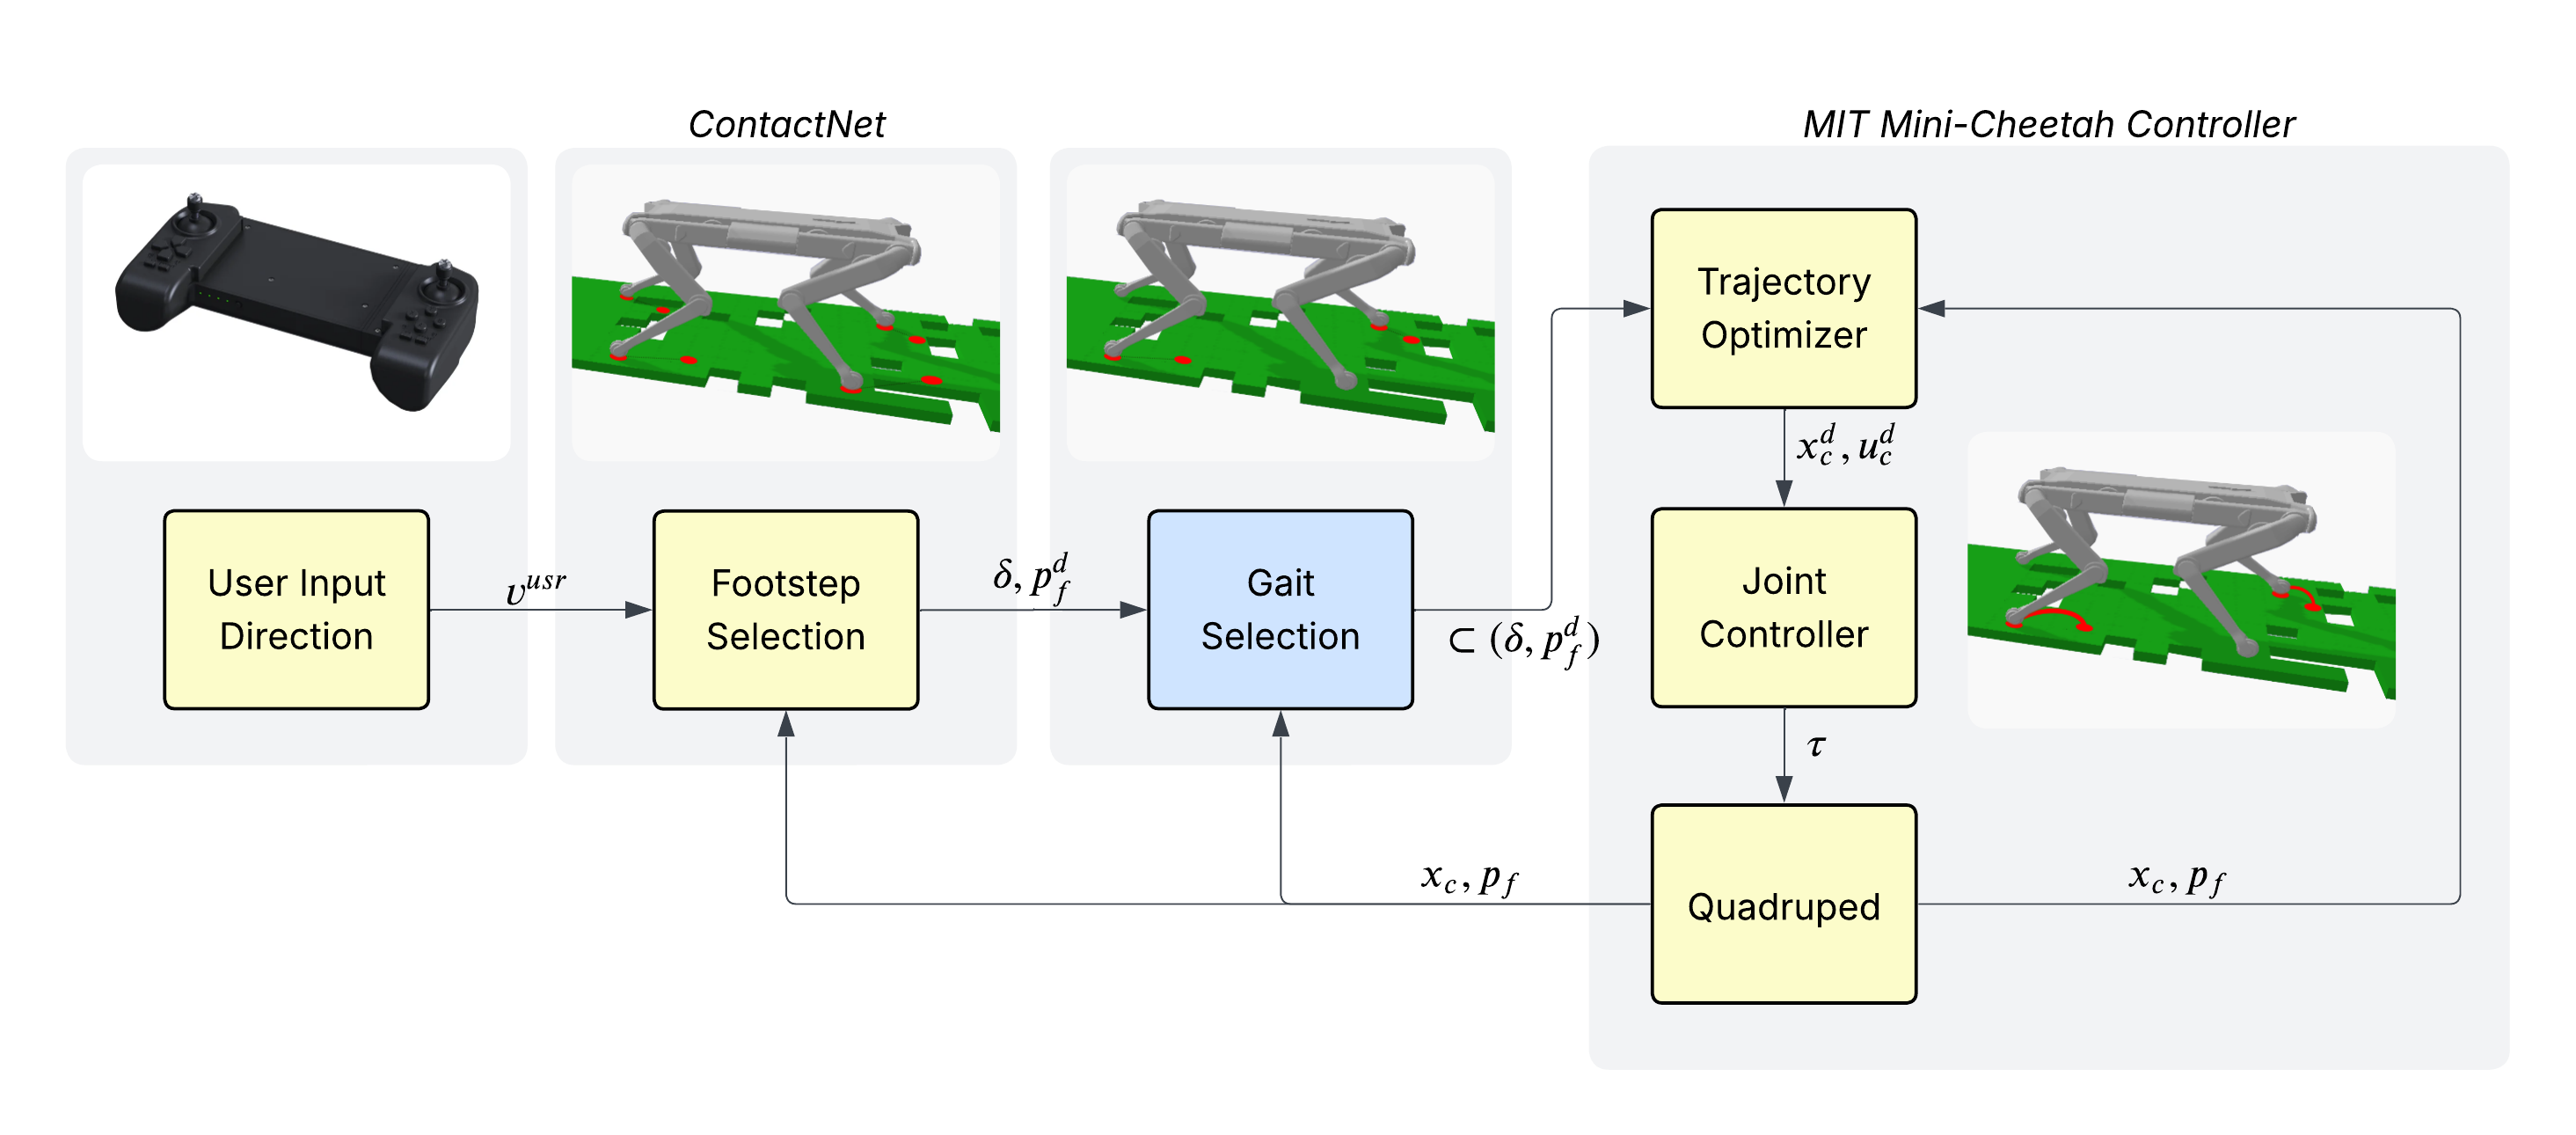
\includegraphics[width=1.0\linewidth]{images/diagrams/control-system.png}
  \caption{A block diagram of the proposed framework. The user defines an input direction $v^{usr}$ which the \textit{footstep selector} \cite{bratta_contactnet_2024} uses along with, the robot state $x_c$, and the current foot positions $p_f$ to generate the swing durations $\delta$ and touchdown points $p_f^d$ for all currently grounded feet. The \textit{gait selector} (novel) takes these desired foot movements and selects an appropriate subset $\subset(\delta,p_f^d)$ based on $x_c$, $p_f$, and the terrain data. $\subset(\delta,p_f^d)$ is then passed into the MIT Mini-Cheetah Controller as MPC constraints to perform lower level control.}
  \label{fig:diagram-control-system}
\end{figure}
